\chapter{Literature Study}
\label{ch:LiteratureStudy}
\graphicspath{{Chapter2/Chapter2Figures/}}

In the previous chapter the problem statement and objectives of this project was laid out. Further, a brief system overview is provided.
This chapter will provide information on already existing Optical Mark Recognition (OMR) systems and the techniques they use for conducting image processing. Research on additional machine learning approaches used in character recognition and probabilistic modelling is also given.

\section{Existing OMR techniques}
An OMR system is software that is used to extracted handwritten information from a filled-in form. Each system normally has a specific template that it can extract information from. An example template is shown in Figure \ref{fig:omrTemplate}. These systems are generally used when fast and accurate grading of tests are required. The main drawback of these systems is that information can only be portrayed in a limited manner, due to the bubbles. On an OMR template there is a grid of bubbles that allows a user to choose between different options to answer. Optical Mark Recognition systems are thus excellent for the grading of multiple choice type questions. 

\begin{figure}
  \centering
  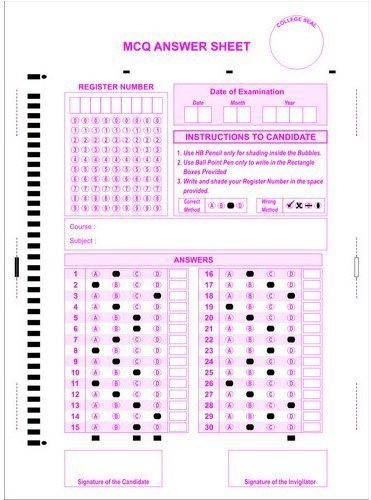
\includegraphics[width=14cm]{omrTemplate}\\
  \caption{Standard OMR template with reference blocks on the left, from \citet{stdTemplate}}
  \label{fig:omrTemplate}
\end{figure}

\subsection{Standard OMR systems}
\label{sec:StandardTech}

As can be seen in Figure \ref{fig:omrTemplate}, there is normally specific reference blocks on an OMR template. These blocks are included to allow the computer vision and image processing algorithms to find the orientation of the image more easily. Other templates include lines that can be used to locate the template.

In an OMR system there are normally two phases in the grading of a test, as stated in \citet{DraganI2003}. The first step is to determine the grid within where the answers are located in the image. In this process the system finds the orientation of the template in the image and therefore can approximate the location of the use of coloured in bubbles. Normally, some preprocessing on a blank template is done beforehand to aid in locating the bubbles. Once the bubbles were found, their estimated locations gets stored. The second step is then to estimate the value of each bubble and use these values as the estimated answers. These steps are described in more detail next.

\subsection{Finding the template}

The first process performed by OMR software is to locate a template grid inside the test image. This step is necessary for the software to identify which bubble corresponds with each answer. One method of locating the template is identifying lines in the template. The border normally contains long lines that can be extracted using a Hough transform (\citet{MVGI2015}). A Hough transform is used to locate instances of an imperfect object within a certain shape range. A specific form of a Hough transform can be implemented to detect lines. This form is called a Radon transform, as described in \citet{MathWorks}. A Radon transform provides a way of representing an image as a summation of different line integrations, as is discussed in Section \ref{sec:RadonTransform}. 

Once at least two line references on a page have been found, the template orientation can be determined. Those two lines are then used to find two reference points on a page. These points allow the system to estimate the locations of every bubble on the template sheet. In the next section a method to process these bubble is described.

\subsection{Processing a bubble}

Once an estimated location for each bubble is known, the next step for an OMR system is to process these bubbles. As stated in \citet{MVGI2015}, a basic image processing method to classify bubbles is to simple add the number of coloured in pixels. If this value is above a specific threshold value, the bubble is classified as filled in, otherwise not. An additional algorithm is needed to detect if a bubble is crossed out .

Contour detection is used to determine if an answer in a bubble is truly coloured in and not just crossed out. This means that the contour around the bubble needs to be detected and used in the analysis. In Python (or C++) this can be implemented using the freely available OpenCV library, as described in \citet{AdrianR2016}. OpenCV is an image processing library that has highly optimized techniques to find contours in a given image. An example of this is shown in Figure \ref{fig:Cross}. Once the contour information is known, the bubbles can be assessed by the pixels inside it, as well as its shape. Thus by looking at the shape of a contour it can be determined if a bubble is crossed out or not.
\begin{figure}
  \centering
  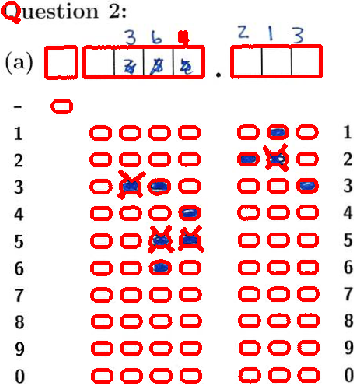
\includegraphics[width=5cm]{Cross}\\
  \caption{Contours found around corrected answer.}
  \label{fig:Cross}
\end{figure}

\section{Optical character recognition}
\nomenclature[A]{$OCR$}{Optical character recognition}
\nomenclature[A]{$DCNN$}{Deep convolutional neural network}
Optical Character Recognition (OCR) software is also needed and applied on the characters blocks present on the templates, to further increase the accuracy of the system. It is found that one preferred way of doing OCR is using TensorFlow. This method is described in \citet{Tensor}. TensorFlow is a Python library, but allows the building of instructions to be implemented in ef{f}icient C++ code. For this test grader, TensorFlow is used to construct a deep convolutional neural network (DCNN). Deep convolutional neural networks are powerful machine learning techniques generally used to process images. One effective application of a DCNN is that it is excellent at processing an image containing a digit and estimating that digit.

\subsection{Probabilistic approach}

A last piece of information that needs to be investigate is how the bubble and character evidence can be brought together in a effective way to produced the best estimate of the intended student entries. Once a bubble and character is analysed, a probabilistic value is assigned to it. Each bubble has a probability of being filled in, while each character has a probability distribution over 10 digits. A probabilistic model is needed to predict these student entries. In \citet{pgmPy}, a machine learning approach is used to infer a probability of random variables being in a certain state given evidence. This method is known as a Probabilistic Graphical Model (PGM). A PGM is a probabilistic framework that consists of a graph that specifies the probabilistic relationship between a number of random variables. These types of models work well in some aspects of the medical field. If a patient has certain symptoms, a PGM can be used to predict what the underlining illness behind the decease is. In this project a PGM can be used to estimate the underling student entries given the evidence presented. The library used in \citet{pgmPy} is called pgmpy. This library allows for a PGM to be constructed in Python. 

\section{Conclusion: System requirements}

In conclusion it is seen that a combination of image processing and machine learning techniques is needed to successfully grade a student test paper. A good method in locating a template is using a Radon transform to find reference lines on an image. Once this is done, the bubbles can be estimated in the image. It is found that a DCNN can be implemented to classified digits in the TensorFlow library space. Once all these evidence are acquired a Probabilistic Graphical Model was found to be a perfected method in predicting the estimated entry answer of the student.
In Chapter \ref{ch:ImageProcessing}, a more detailed overview on the image processing techniques used in this project is given.
